\documentclass{sig-alternate-05-2015}

\usepackage{hyperref}
\usepackage{xcolor}
\usepackage{xeCJK}

\hypersetup{
    colorlinks,
    linkcolor={red!50!black},
    citecolor={blue!50!black},
    urlcolor={blue!80!black}
}

\begin{document}
\title{Predicting Censorship on Weibo}
\subtitle{CSE 190: Assignment 2}

\numberofauthors{2}
\author{
  \alignauthor
  Brian Tsay \\
  \email{brtsay@ucsd.edu}
  \alignauthor
  John Kuk \\
  \email{jskuk@ucsd.edu}
}

\date{1 December 2015}

\maketitle

% don't forget abstract
\begin{abstract}
  Put abstract here.
\end{abstract}


 \begin{CCSXML}
<ccs2012>
<concept>
<concept_id>10010405.10010455</concept_id>
<concept_desc>Applied computing~Law, social and behavioral sciences</concept_desc>
<concept_significance>300</concept_significance>
</concept>
</ccs2012>
\end{CCSXML}

\ccsdesc[300]{Applied computing~Law, social and behavioral sciences}
\printccsdesc

\section{Dataset} \label{sec:data}
% need time series plot
The data used for this assignment is taken from the \href{http://weiboscope.jmsc.hku.hk/datazip/}{Weiboscope} data collection and visualization project developed by the research team at the Journalism and Media Studies Centre, The University of Hong Kong \cite{Fu2013a}. The dataset consists of weibos (roughly the Chinese equivalent of tweets) collected in the year 2012. The authors created the dataset by first compiling a list of Weibo users with 1,000 or more followers and then getting their timelines, friends, and followers. Within the entire dataset, there are 226,841,122 tweets from 14,387,628 unique users. Of these tweets, 86,083 (about 0.03\%) are censored.

\begin{figure*}
  \centering
  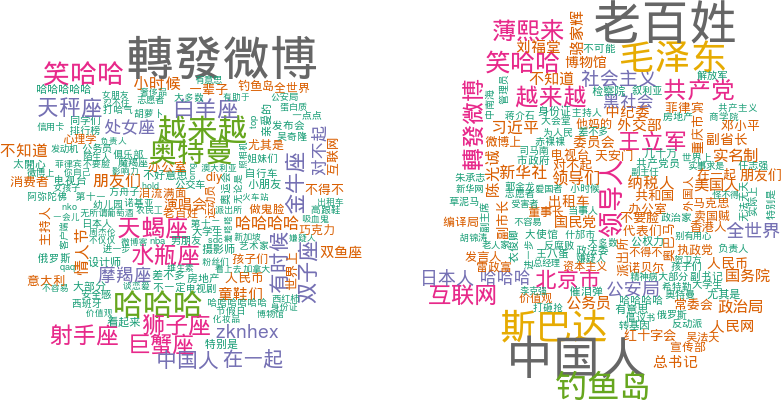
\includegraphics[scale = 0.65]{wc.png}
  \caption{Noncensored (Left) and Censored (Right) Tweets Word Cloud}
  \label{fig:wordcloud}
\end{figure*}

Figure~\ref{fig:wordcloud} shows the word clouds for the noncensored tweets (left) and for the censored tweets (right). Some terms are found often in both sets, namely 轉發微博 (retweet), 哈哈 (haha), 中国人 (Chinese people), and 越来越 (more and more). 

However, censored tweets tend to be much more political. 钓鱼岛 (Diaoyu Islands) refer to the disputed island chains between China and Japan. 斯巴达 (Sparta) is actually a play on the fact that Sparta in Chinese (sibada) is nearly a homophone for 十八大 (shibada), the 18th National Party Congress where the previous president Hu Jintao stepped down and the current president -- Xi Jinping -- took his place.\footnote{Chinese internet users often rely on homophone tricks such as these to evade automatic keyword censoring. In this case, we can see that it was not 100\% effective.} There tend to be more people names in the censored tweets, such as 毛泽东 (Mao Zedong, former chairman of the Chinese Communist Party), 薄熙来 (Bo Xilai, disgraced Chongqing party chief), 王立军 (Wang Lijun, vice-mayor of Chongqing under Bo), and others. There are also references to the Chinese government, such as 领导人 (leadership) and 共产党 (Communist Party), and the masses (老百姓).

In comparison, the noncensored tweets appear much more benign. One of the most common terms is 奥特曼, which refers to the fictional Japanese superhero Ultraman, who is apparently quite popular among a certain generation in China. Many popular terms are simply astrology zodiac signs e.g. Leo (狮子座), Sagittarius (射手座), etc. The astrology most likely comes from a bot or person that tweets horoscopes every day.\footnote{Astrology is actually fairly \href{https://newrepublic.com/article/119500/chinese-astrology-surprising-prominence-horoscopes}{popular in China}.} The popularity of the term Ultraman can perhaps be attributed to the creation of a noodle-robot that looked \href{http://asiasociety.org/blog/asia/video-when-going-gets-tough-superhero-robot-turns-noodle-making}{like Ultraman in 2012}. The conclusion would be that we should look for more overtly political words to classify censored tweets.

For the assignment, we kept all the censored tweets but kept only a small subsample (0.1\%) of the noncensored tweets. Noncensored tweets were randomly sampled from the entire dataset such that the number of noncensored tweets would be roughly twice that as the number of censored tweets within our data.\footnote{There was no particular reason that this ratio was chosen.} Whereas 0.03\% of tweets are censored in the entire dataset, 34\% of tweets are censored in our small subsample. The training set was constructed such that half of the tweets would be censored while the other half would be noncensored. The validation and test sets were deliberately constructed to look like one another. 

\begin{table*}
  \centering
  \begin{tabular}{|l|c|c|c|c|}
    \hline
    Statistic & Training Set & Validation Set & Test Set & Total \\
    \hline
    Retweets & 47930 & 41285 & 41414 & 130629 \\
    Unique Users & 39719 & 50446 & 50620 & 107907 \\
    \hline
    Censored Tweets & 43042 (50\%) & 21521 (25\%) & 21521 (25\%) & 86084 (34\%)  \\
    Non-censored Tweets & 43042 (50\%) & 63291 (75\%) & 63292 (75\% )& 169625 (66\%) \\
    Total Tweets & 86084 & 84812 & 84813 & 255709 \\
    \hline
  \end{tabular}
  \caption{Dataset Statistics}
  \label{tab:descript}
\end{table*}

Table~\ref{tab:descript} shows some descriptive statistics for our dataset. It appears that more than half of the tweets in our subsample are retweets.\footnote{Note that this is a function of how the original dataset was constructed. This is not an artifact of our random sampling strategy.} We also see that, on average, each user is producing 2.5 tweets in our dataset. This implies that many tweets are correlated with one another. A retweet is very likely related to whatever the original tweet was, and individual users will probably tweet similar things over time. These aspects of the data will be incorporated into our features as described in Section~\ref{sec:pred}.

\begin{figure}
  \centering
  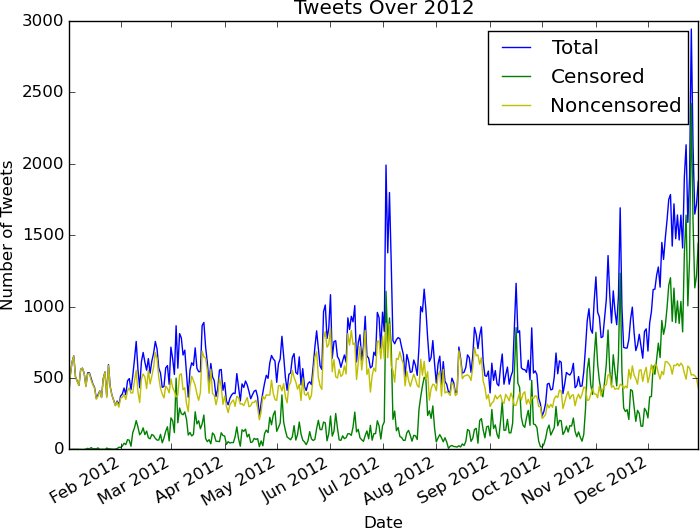
\includegraphics[scale=0.5]{tweetTime.png}
  \caption{Tweets over Time}
  \label{fig:ts}
\end{figure}

Figure~\ref{fig:ts} shows the distribution of tweets over time in our small subsample. While the number of noncensored tweets is somewhat constant over time, the number of censored tweets clearly vary greatly over time. There are few censored tweets in the beginning of the year, with a spike coming in mid-2012 and a huge increase near the end of 2012. The spike at the end corresponds to the 18th Party Congress mentioned above. The spike in the summer of 2012 roughly corresponds to anti-Japanese protests held in multiple Chinese cities. A good predictive model should therefore require some way to account for the temporal aspect of censorship. 

In other words, there are many factors at play in determining whether a tweet is censored or not. How we explicitly model these factors will be explained in the following section.

\section{Predictive Task} \label{sec:pred}
We would like to predict which tweets are censored in this dataset i.e. a binary-class prediction. To evaluate our model, we will simply use classification accuracy -- the proportion of tweets that are labelled correctly. If we were Chinese government censors, then perhaps we would evaluate recall or $F_\beta$ instead.\footnote{Recall that $F_\beta = (1+\beta^2) \cdot \frac{\text{precision} \cdot \text{recall}}{\beta^2 \text{precision} + \text{recall}}$} The idea is that a government censor would prefer flagging a ``harmless'' tweet for censorship over accidentally letting a ``harmful'' tweet through. We are [fortunately] not Chinese government censors, so we will stick with evaluating our model using classification accuracy. 

Our data are split into training, validation, and test sets using the procedure described in Section~\ref{sec:data}. We purposely oversampled censored tweets (by including literally all of them) in our training, validation, and test sets. This oversampling makes sense for the training set, since we want a balanced sample to be used for training the model. This also certainly made the predictive task easier, since a trivial predictor -- one that predicts no tweets are censored -- on the entire dataset would have been 99.97\% accurate while only 75\% accurate on our test set. 

The features we chose to include in our model can be categorized into two types: the actual text of the tweet and metadata about the tweet. For the text, we either used a simple bag-of-words representation with term frequency-inverse document frequency (tf-idf) weighting or a latent Dirichlet allocation (LDA) topic model to represent each tweet. 

Processing Chinese text data is not exactly the same as processing English text. One of the major differences is that there are no spaces in Chinese text, so spaces must first be inserted between words in each document before a bag-of-words representation can be made. This process is known as segmentation. 

Another major difference between Chinese and English is that Chinese is a ideogram-based language while English is an alphabet-based language. This creates problems for determining where to insert spaces. Consider the following example. The word 電 means electric and the word 腦 means brain. However, combining the two words yields 電腦, which means computer.

The segmentation task therefore becomes a machine learning problem where the model tries to predict what type of $n$-gram a word is. When the segmenter encounters a word like 電腦, it must decide whether this is a bigram (computer) or two unigrams (electric brain).\footnote{This example is somewhat stupid since it's unlikely for anyone to be talking about electric brains, but the basic point still stands.} We had our hands full with our actual predictive task, so we used the basic Chinese segmenter provided in the \href{http://nlp.stanford.edu/software/segmenter.shtml}{Stanford Word Segmenter} \cite{Chang2008}. After segmentation, we removed punctuation and numbers.

One baseline we can then use is just the bag-of-words representation of each tweet, with all 229,334 terms and tf-idf weighting. The baseline accuracy for this simple representation is 76.23\% on the validation set, only slightly better than the trivial predictor (75\% accuracy).

In an attempt to capture latent topics underlying tweets, we use LDA to express tweets as a mixture of topics. These topics do appear to have captured relevant terms. For example, with 50 topics, the three highest-weighted topics can be seen in table~\ref{tab:lda}. As can be seen the highly-weighted topics correspond to sensitive or political terms.

\begin{table*}
  \centering
  \begin{tabular}{l|l|l}
    1 & 2 & 3 \\
    \hline
    link (holder to replace URLs) & 人民 (people) & 国家 (nation) \\
    书记 (secretary) & 政府 (government) & 领导 (leader) \\
    网友 (netizen) & 网络 (network) & 官员 ([government] official)\\
    中央 (central) & 重庆 (Chongqing) & 政治 (politics )\\
    要求 (demands) & 警察 (police) & 公开 (open) \\
    调查 (inspect) & 日报 (times [newspaper]) & 财产 (financial assets) \\
    干部 (cadre) & 法律 (law) & 公布 (publicize) \\
    信息 (information) & 群众 (masses) & 百姓 (common people)\\
    发表 (issue) & 行为 (behavior) & 老百姓 (common people) \\
    十八 (18) & 公安 (public security) & 体制 (system) 
  \end{tabular}
  \caption{Highest-Weighted Topics, $k$=50}
  \label{tab:lda}
\end{table*}


We also incorporate metadata about the tweets (user information, time information, etc.) into our features. We created the following feature vector from \textbf{only} the training data:
\begin{enumerate}
\item The proportion of the user's tweets that have been censored.
\item The number of the times the user has been retweeted.
\item The number of the times the tweet has been retweeted.
\item The proportion of tweets that were censored that day.
\item The proportion of the retweeted user's tweets that have been censored, given that the tweet is a retweet.
\end{enumerate}
There used to be a sixth feature that indicated the number of times that a retweeted message has been censored. However, since our subsample is only a tiny subset of the entire dataset, this value was always 0.

We create these features for the following reasons. A user who is censored more is likely to tweet things that are flagged for censorship (both in our dataset and in the future). Censors are more likely to care about popular tweets and users -- which tend to mean a greater audience -- than they care about unpopular tweets and users, who less people are likely to see. There are certain days (time periods) where there is some event that leads to greater discussion on Weibo and in turn greater censorship by the authorities. 

When we train using only these features, we get a surprising baseline 93.19\% accuracy on the validation set. This strange result will be discussed in Section~\ref{sec:res}. 

\section{Model}
For this binary classification task, we didn't do anything fancy; we used L2-regularized logistic regression and SVM as implemented in the \textsf{LIBLINEAR} library \cite{Fan2008}. For SVM, we did not use any kernel (like the ones provided in the \textsf{LIBSVM} library) since we wanted to keep training time short. A linear classifier is particularly appropriate for our bag-of-words representations, where both the number of instances and features are fairly large. With such a high-dimensional feature space, it is unlikely that mapping such data into even higher-dimensional space would have yielded increases in accuracy.

\begin{figure}
  \centering
  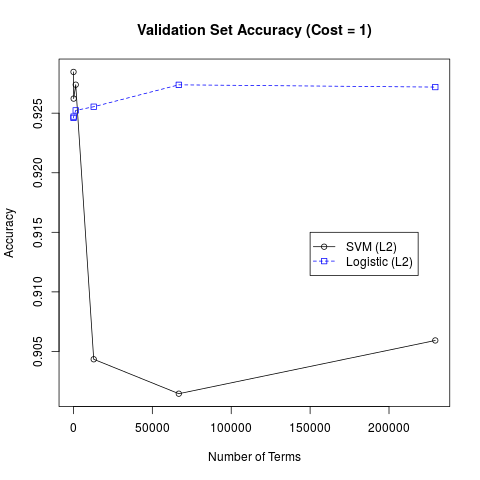
\includegraphics[scale=0.5]{valid_numTerms.png}
  \caption{Tuning Bag-of-Words Sparsity}
  \label{fig:sparse}
\end{figure}

Ideally we would have used grid search or something more rigorous to tune our hyperparameters (the number of terms for bag-of-words and the number of topics for LDA). Instead, we optimized the number of terms and topics first while setting the cost $C=1$. We then fixed the number of topics and terms to the ``optimum'' settings derived from the previous step and then allowed cost to vary.

When the bag-of-words representation for text was initially created, it contained 229,334 terms. We hypothesize that many of these terms might be completely useless or even detrimental to the model by inducing overfitting. We therefore attempted some dimension reduction via just dropping infrequent terms and by applying LDA (discussed later). Infrequent terms were removed based on their sparsity, using maximum allowed sparseness values of 0.99, 0.995, 0.999, 0.9999, 0.99999, and 1 (all terms included). These correspond to 48, 141, 1451, 12849, 66771, and 229334 terms, respectively. Figure~\ref{fig:sparse} shows the results from tuning the number of terms to include in the basic bag-of-words representation of tweets. 

Indeed, there is a small reduction in error on the validation set when we reduce the number of terms. The accuracy for SVM is maximized when we include 1,451 terms instead of the full 229,334 terms. The accuracy for logistic regression is maximized when we have 12,849 terms.

\begin{figure}
  \centering
  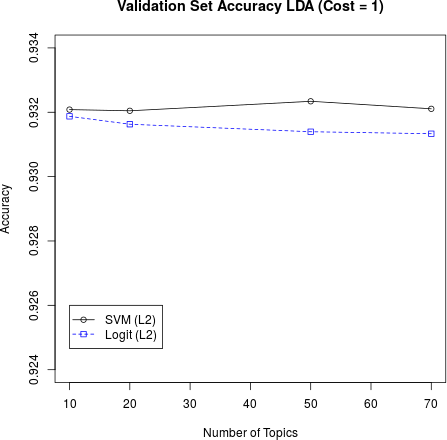
\includegraphics[scale=0.5]{valid_k.png}
  \caption{Tuning LDA Topics}
  \label{fig:LDA}
\end{figure}
The results from tuning the number of topics $k$ is shown in Figure~\ref{fig:LDA}.

The costs are imposed on the logistic regression and SVM models to prevent overfitting. For both, the cost $C$ is applied in the following optimization problem
\begin{equation}
  \label{eq:svm}
  \min_w \frac{1}{2} \mathbf{w}^T\mathbf{w} + C \sum_{i=1}^l \xi(\mathbf{w}; \mathbf{x}_i; y_i)
\end{equation}
where $\mathbf{w}$ refers to the weight vector, $(\mathbf{x}_i$, $y_i)$ is the set of instance-label pairs for $i=1, \ldots, l$, and $\mathbf{x}_i \in R^n$ and $y_i \in \{-1,1\}$. The loss function $\xi(\cdot)$ is $\max(1-y_i\mathbf{w}^T\mathbf{x}_i,0)^2$ for L2-SVM and $\log(1+e^{-y_i\mathbf{w}^T\mathbf{x}_i})$ for L2-logistic regression. For SVM, the cost $C$ represents the tradeoff between maximizing the margin on the training set (overfitting?) and minimizing the classification error. For logistic regression, the cost $C$ penalizes overly large (in magnitude) weight vectors.

The results from tuning the cost parameters are shown in Figure~\ref{fig:cost}. Most of the models have very similar accuracies, which is unsurprising given the fact that much of the models' predictive power comes from the meta features. The best performance seems to be achieved for costs between 0.001 and 100, though the differences are slight. SVM tends to experience a relatively large dropoff in accuracy for costs of 100 and above, perhaps implying that accuracy is being sacrificed to maximize the margin. Logistic regression doesn't seem to experience these effects, perhaps implying that the weights were not growing large in magnitude to begin with. Lower costs also hurt logistic regression relatively more than SVM, perhaps implying that at least some overfitting on the training set is occurring. It should be noted that tuning the cost actually does very little in absolute terms, since the difference in accuracy rate is generally around 0.01\%, corresponding to roughly 80 tweets in our validation set.

\begin{figure}
  \centering
  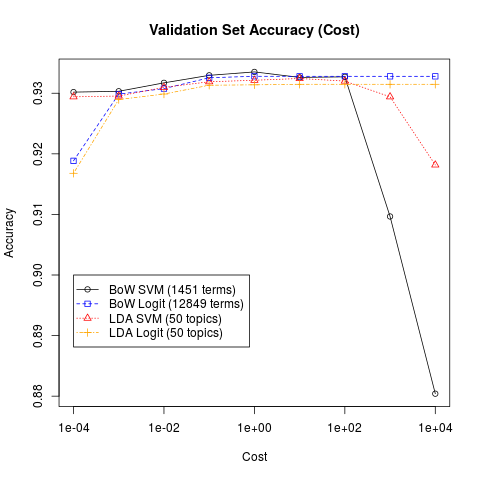
\includegraphics[scale=0.5]{valid_cost.png}
  \caption{Cost Tuning}
  \label{fig:cost}
\end{figure}

\section{Literature}

The development of text mining has opened a new research topic in studying Chinese government censorship on social media. To study censorship existing studies use microblogs like Weibo \cite{bamman2012censorship, Fu2013a}, Chinese language messages from Twitter \cite{bamman2012censorship}, or blogs \cite{king2013censorship}. The main difference between existing studies and our study is the research goals. Existing studies try to answer what words \cite{bamman2012censorship, Fu2013a} or themes \cite{king2013censorship} are the targets of censorship. Even they collect every message they scrap, only deleted messages are the scope of their analysis. These studies find that politically sensitive words are likely to be deleted \cite{bamman2012censorship, Fu2013a}. Further analyzing what politically sensitive words and topics mean, it is found that government criticisms are relatively allowed compare to messages that have collective action potential \cite{king2013censorship}. The findings from existing studies imply using text would be powerful to predict what message is going to be censored, but they did not analyze prediction on censored / non-censored messages including other features in the model. 

Existing studies could be done because of data collection strategy. All of these studies revisit their target websites multiple times to detect government censorship. To compare the relative frequency of each keyword occurrence in censored and uncensored messages, $\chi^2$ feature selection algorithm to calculate the relative frequency is used \cite{Fu2013a}. Using keywords to predict censorship is intuitive, but this method lacks contexts for each keyword. To overcome this problem, classifying documents by content area using supervised model is the state-of-the art method in this area of research. To classify massive of amount of data, multiple human coders classify a sample of documents and make the model aggregate and classify the remaining documents \cite{king2013censorship}.\footnote{King et al. 2013 \cite{king2013censorship} uses ReadMe \cite{hopkins2010method} method which is a non-parametric approach for characterizing distribution of classes. It requires fewer assumptions than other methods. Especially, it does not need random sample of documents. Without making Naive Bayes like assumption, this algorithm examines joint distribution of characteristics  and focuses on distributions makes this analysis possible.} Our paper was motivated by the fact that the newest research on this topic considers content area and topic seriously.


\section{Results} \label{sec:res}
\begin{table}
  \centering
  \begin{tabular}{l|c}
    Model & Test Accuracy \\
    \hline 
    BoW 1451 + Meta (SVM, C=1) & 93.33\% \\
    BoW 12891 + Meta (Logit, C=1) & 93.28\% \\
    BoW all only (Logit, C=1) & 73.42\% \\
    LDA 50 + Meta (SVM, C=1) & 93.19\% \\
    LDA 10 + Meta (Logit, C=1) & 93.14\% \\
    LDA 10 only (Logit, C=1) & 74.44\% \\
    Meta only (Logit, C=1) & 93.10\% \\
    Trivial predictor & 75\%
  \end{tabular}
  \caption{Results}
  \label{tab:results}
\end{table}
Results are seen in Table~\ref{tab:results}. 

The main issue is the fact that our baseline using only the meta features of a tweet is so high. One potential reason for this is the fact that we included too many censored tweets in our training set. By including 50\% of all the censored tweets in the entire 220 million tweet dataset within the training set, we may have given the model too much meta information to work with. The major drivers behind the high accuracy are the first (proportion of user's tweets that have been censored) and fifth (proportion of retweeted user's tweets that have been censored) features. In terms of online/real-time learning, these features are slightly unrealistic, since they allow us to sort of ``see into both the past and future'', since these tweets cover the entirety of 2012. 

\bibliographystyle{abbrv}
\bibliography{writeup}

\appendix
Code for this project can be found on our \href{https://github.com/brtsay/CSE190_Assignment2}{Github page}.
\end{document}
